%%% maw.tex
\section{Minimal Absent Words and Maximal Repeats}

We introduce a fundamental concept of maximal repeats of a string $S$, which is useful for realizing efficient enumeration of many kinds of unusual words. Then, we give a characterization of the set $\MAW(S)$ of minimal absent words of a string $S$. 
Let $S = S[1..n] \in \Sigma^n$ be a string over alphabet $\Sigma$ and $\hat S[0..n+1] = \# S\daller \in \hat\Sigma^{n+2}$ be its extended version with endmarkers.

%%%% 
\mysubsubsection{Maximal repeats}
%%%%
A repeat of $S$ is any substring $u \in \Sigma^+$ that occurs at least twice in $S$, that is, $u \in \Fac(S)$.
Let $u \in \Sigma+$ be any factor of $\hat S$. Since $\#, \daller \not\in \Sigma$, we see $u \in \Fac(S)$, namely, $u$ is contained in the content $S$.
%%% 
%% \begin{definition}[maximal repeat]\rm 
A string $u \in \Sigma+$ is a \textit{maximal repeat} of $S$ if it satisfies the following conditions: 
\begin{enumerate*}[(1)]
\item $u$ is a factor of $S$, i.e., $u \in \Fac(S)$;  
\item there exist two start positions $p, q \in \Spos[S](u)\;(p\not= q)$ of $u$ such that
  \begin{enumerate*}[(i)]
  \item $u$ is \textit{left-branching} meaning that the preceding characters are mutually different, i.e., $S[p-1] \not= S[q-1]$, and
  \item $u$ is \textit{right-branching} meaning that the following characters are mutually different, i.e., $S[p+|u|] \not= S[q+|u|]$. 
  \end{enumerate*}
\end{enumerate*}
%% \end{definition}
In what follows, $\MR(S)$ denotes the set of all maximal repeats of a string $S$. By definition, any $w$ in $\MR(S)$ correctly occurs at least twice in $S$. 

For later use, we define the \textit{set of left characters} $\LSigma(u) \subseteq \Sigma\cup\set{\#}$ (resp.~\textit{right characters} $\RSigma[](u) \subseteq \Sigma\cup\set{\daller}$) of a factor $u \in \Fac(S)$ to be the sets of all characters $S[p-1] \in \hat\Sigma$ (resp.~$S[p+|u|] \in \hat\Sigma$) preceding (resp.~following) all positions $p\in \Spos(u)$ of $u$ in $\hat S$.
If it is clear from context, we write $\LSigma[](u)$ and $\RSigma[](u)$ by omitting subscript $\hat S$. 
Using this notation, we can redefine a maximal repeat of $S$ to be any nonempty string $u \in \Fac(S)$ with $|\LSigma(u)| \ge 2$ and $|\RSigma(u)| \ge 2$.


\mysubsubsection[]{Minimal absent words}
%%%% 
%A \textit{minimal absent word} (MAW)
of a string $S$ are a class of unusual words, introduced by Garcia, Pinho, Rodrigues, Bastos, and Ferreira~\cite{garcia2011minimal}. A \textit{MAW} is a non-trivial string $w$ that does not occur in $S$, and any proper factor of $w$ occurs in $S$ as a substring (see \cite{garcia2011minimal}).
Precisely, a MAW of $S$ is a string $a u b$ with $a, b\in \hat\Sigma$ and $u \in \Sigma^+$ such that
\begin{enumerate*}[(i)]
\item $w \not\in \Fac(\hat S)$; and 
\item $au, ub \in \Fac(\hat S)$. 
\end{enumerate*}

As an example, the minimal absent words of the string $S = \texttt{aabaababb}$ are shown in \cref{fig:example:maw}. 

%%%%%%
\begin{figure}[t]
\centering  
%% 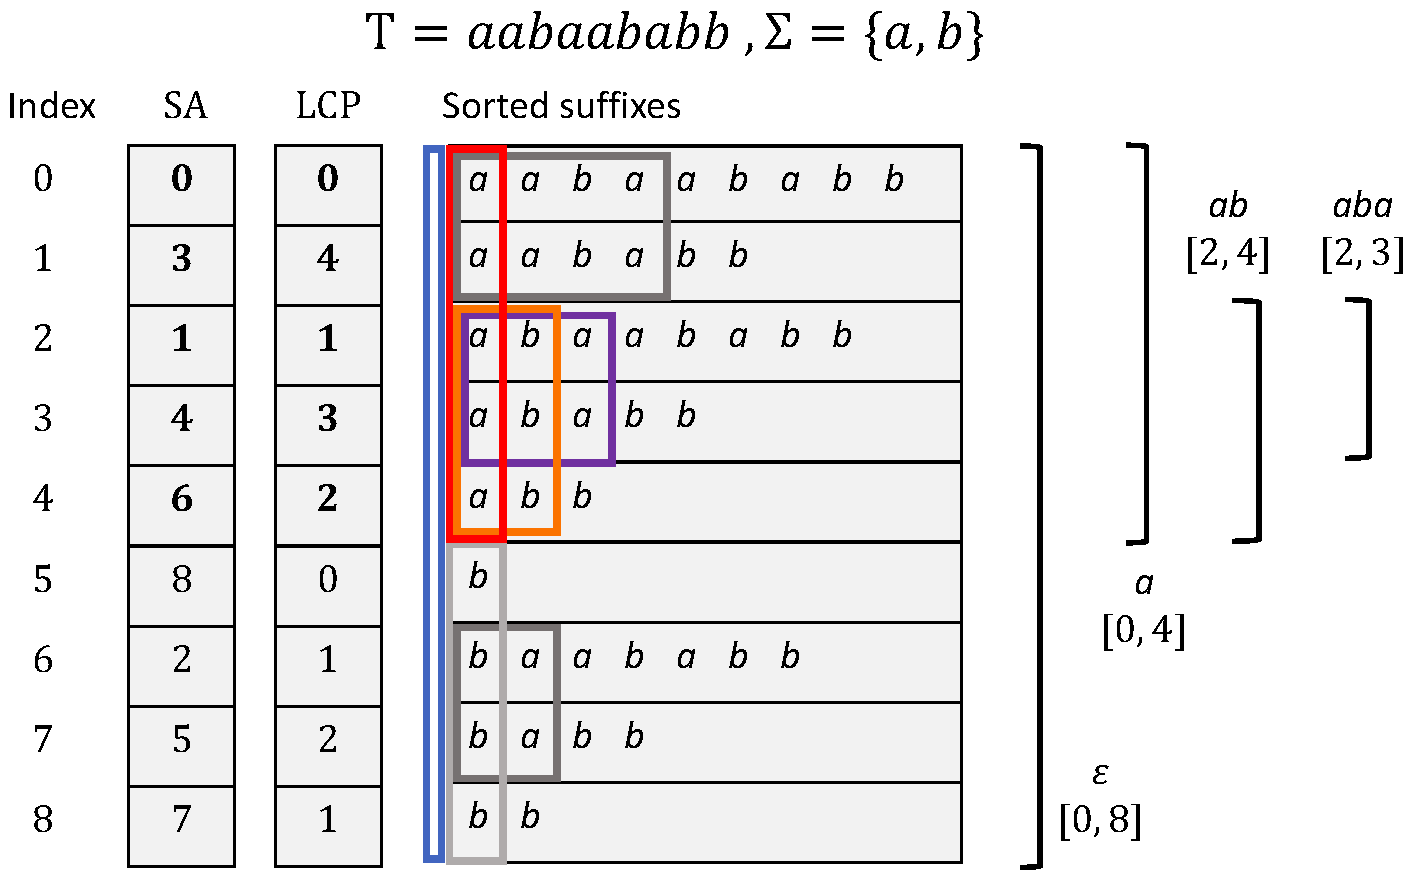
\includegraphics[width=0.60\textwidth]{fig/exp1/fig1.pdf}
\vspace{.5\baselineskip}
\caption{An example of minimal absent words of the string $S = \texttt{aabaababb}$. 
}\label{fig:example:maw}
\end{figure}
%%%%%%

%%% EOF
